\epigraph{Nature folds to densify --- from the brain to the universe.}{}

\section{The Deformation}


\begin{figure}[ht]
\centering
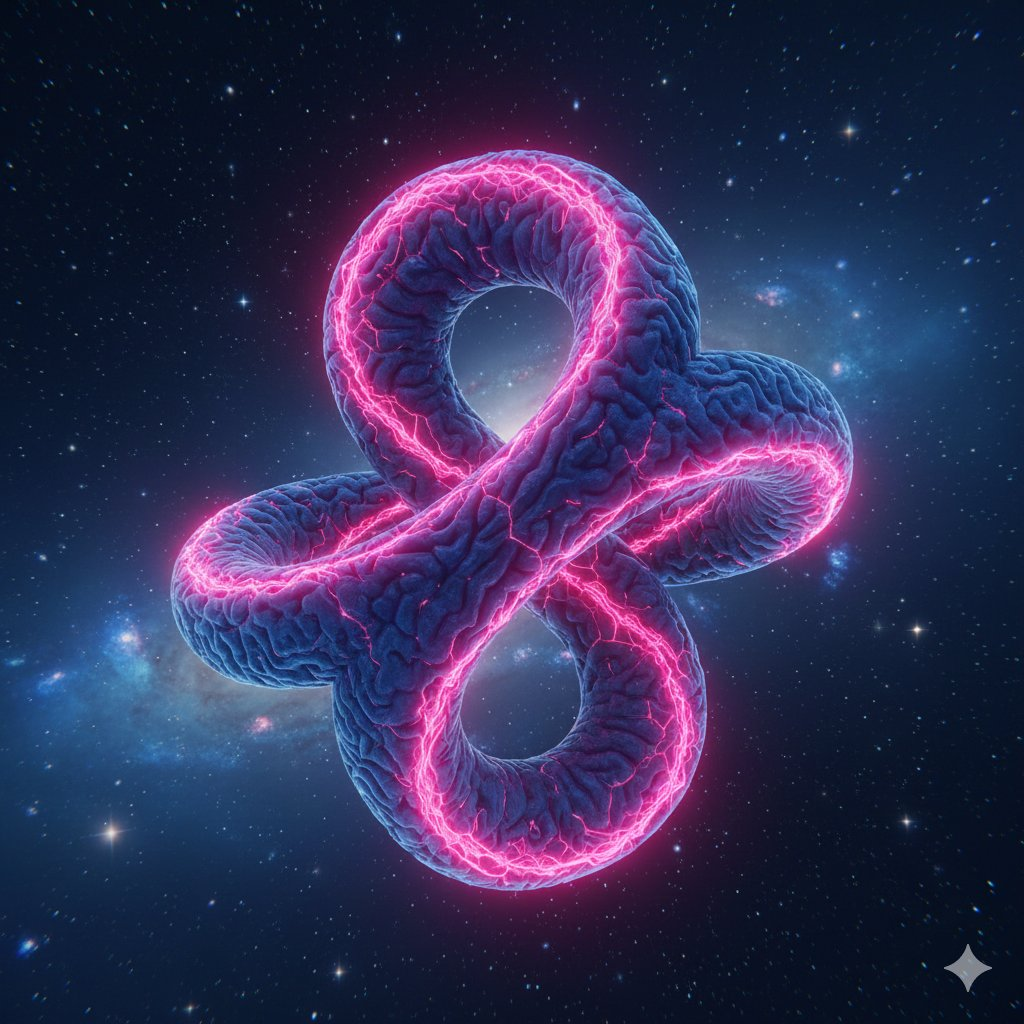
\includegraphics[width=0.75\textwidth]{img/brain_torus_artistic.png}
\caption{Artistic depiction of a brain-like torus: a folded tube with gyrus-like surface texture, threaded by energy flow lines. The idea is analogous to DNA: just as the double helix compacts via nucleosomes, solenoid loops, and chromatin fibres into a dense chromosome, one can imagine the brain-fold torus as a similar hierarchical condensation --- a long, thin energy tube that folds upon itself at ever tighter scales until the furrowed, brain-like surface emerges. \emph{Note:} This is a highly simplified, artistic visualisation --- the image illustrates the principle, not anatomical accuracy.}
\label{fig:brain_torus}
\end{figure}
The ideal, smooth torus is a starting point but not the end of the story. In physical reality the torus deforms into a \textbf{brain-fold torus} --- a topology reminiscent of the gyri and sulci of the cerebral cortex.

The analogy is not accidental. The human brain solves a fundamental geometric problem: how does one maximise surface area (and thus processing capacity) within a bounded volume? The answer of biological evolution: through folding. The cerebral cortex folds into convolutions (gyri) and grooves (sulci), multiplying its surface area many times over. That nature finds the same geometric solution at the most fundamental and the most complex level is, in the T0 perspective, no coincidence --- it is geometric necessity (see Chapter~16).

Nature chooses the same solution at the most fundamental level. The four-dimensional torsion crystal folds into a convolution mesh in which the \emph{interaction surface} is dramatically enlarged --- while the volume remains finite.

\section{Particles as Resonances}

In this picture elementary particles are not point-like objects and not excitations of an abstract quantum field. They are \textbf{standing waves} --- resonances in the convolution mesh of the torus. An electron is a particular resonance mode, a muon another, a tau a third. The three generations of particle physics correspond to three different resonance modes of the same geometric object.

The forces between particles are \textbf{geometric couplings} between different torsion modes. Electromagnetism, the weak and strong forces --- they all describe how different resonances in the convolution mesh interact with one another. And the masses of the particles are the \textbf{frequencies} of these resonances (cf.\ \href{https://github.com/jpascher/T0-Time-Mass-Duality/blob/main/2/pdf/006_T0_Teilchenmassen_De.pdf}{Doc.~006}, \href{https://github.com/jpascher/T0-Time-Mass-Duality/blob/main/2/pdf/046_Teilchenmassen_De.pdf}{046}, \href{https://github.com/jpascher/T0-Time-Mass-Duality/blob/main/2/pdf/116_T0_koide-formel-3_De.pdf}{116} for the mass calculations).

\section{The Winding Number and $\xsi$}

The winding density directly determines the parameter~$\xsi$: with $30000/4 = 7500$ windings one obtains $\xsi = 4/30000$. This is the bridge between abstract geometry and the measurable parameter.

\section{What the Brain-Fold Torus Explains}

The folded torus structure provides explanations for three central puzzles:

First: \emph{Why are there exactly three generations?} Electron, muon, and tau are not arbitrary copies of the same particle. They are the three lowest resonance modes of the convolution mesh --- comparable to the fundamental tone and the first two overtones of a string.

Second: \emph{Why the hierarchy problem?} The enormous difference between the Planck energy and the electroweak scale has a geometric cause: the Planck energy distributes across $f^4$ cells in the four-dimensional hypercube of the torus structure. $7500^4 \approx 3.16 \times 10^{15}$ --- precisely the order of magnitude of the hierarchy problem.

Third: \emph{Why the gravitational constant is so small.} $G$ scales with~$\xsi^2$, and $\xsi$ is the inverse winding number. More windings mean finer torsion, and finer torsion means weaker effective gravitation.

\section{Time in the Torus}

Here lies perhaps the conceptually most difficult point: the torus encodes \emph{time as well}.

In standard physics one thinks in three spatial dimensions plus a separate time dimension. In T0, time is not an external coordinate. It is \emph{woven into the torus structure} --- as the phase evolution~$\theta(x)$ of the vacuum field.

The phase~$\theta$ of the vacuum field~$\Phi = \rho \cdot e^{i\theta}$ \emph{is} time: $\dot{\theta} = m = 1/T$. Time is not something that ``passes'' --- it is the \emph{rotation rate} of the torus.

The local time rate corresponds to the local winding speed of the torus phase. Where more mass is present (higher~$\rho$), the phase rotates more slowly --- that \emph{is} time dilation. Where there is less mass, the phase rotates faster --- that \emph{is} the faster time in the vacuum.

Time-mass duality~$T \cdot m = 1$ is, in this picture, not a postulate but \emph{geometric necessity}: winding frequency times inertia equals a constant on the torus.

\begin{kerngedanke}
The torus is hard to visualise because we experience time as a ``flow.'' But physically, time is a phase coordinate on a closed manifold --- no more fundamental than the angle on a circle.
\end{kerngedanke}
